\begin{frame}
    \centering \Huge
    NCCL
\end{frame}

\begin{frame}{NCCL - Comunicazione collettiva GPU}
    \begin{itemize}
        \item Libreria NVIDIA per comunicazioni collettive ad alte prestazioni tra GPU.
        \item Supporta ambienti multi-GPU e multi-nodo.
        \item Primitive principali: \texttt{broadcast}, \texttt{reduce}, \texttt{all-reduce}, \texttt{all-gather}, \texttt{reduce-scatter}.
        \item Sfrutta interconnessioni NVLink, PCIe, InfiniBand.
    \end{itemize}
\end{frame}

\begin{frame}{Architettura NCCL}{Comunicazione Peer-to-Peer}
    \begin{itemize}
        \item Comunicazioni dirette GPU-GPU (peer-to-peer), evitando la CPU.
        \item Topologia costruita dinamicamente in fase di inizializzazione.
        \item Supporto per NVLink, PCIe, SHMEM (intra-nodo), UCX (inter-nodo).
        \item Coordinamento tramite topologie a \textbf{ring} e \textbf{albero}.
    \end{itemize}

    \begin{figure}
        \centering
        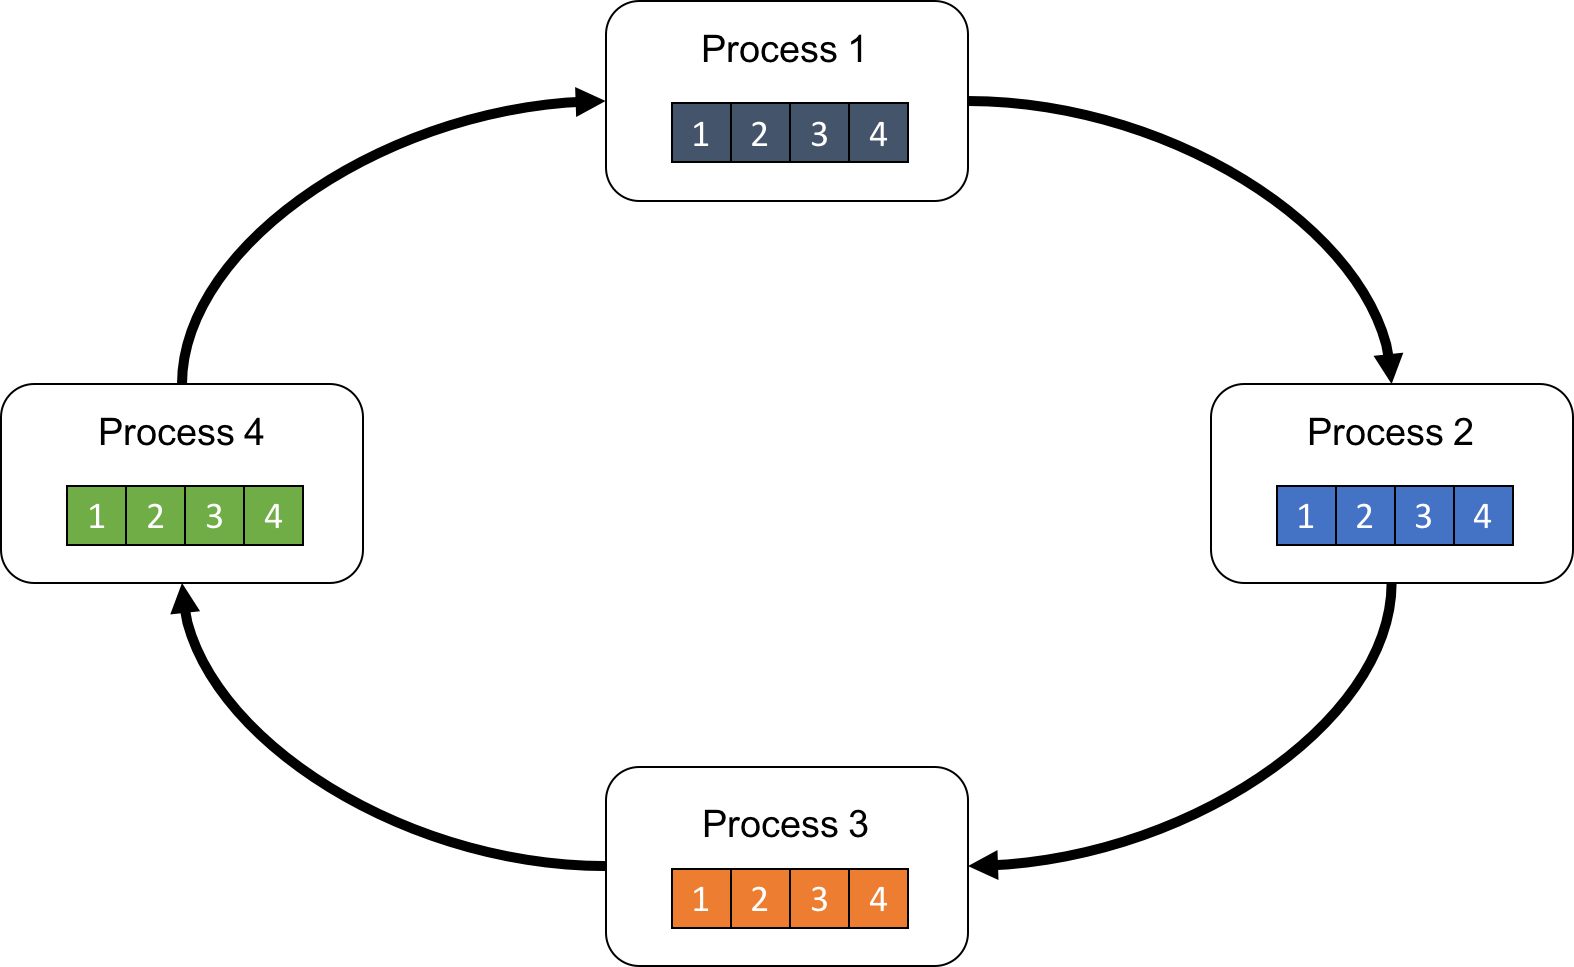
\includegraphics[width=0.48\textwidth]{imgs/nccl_topology_ring_tree.png}%
        \hfill
        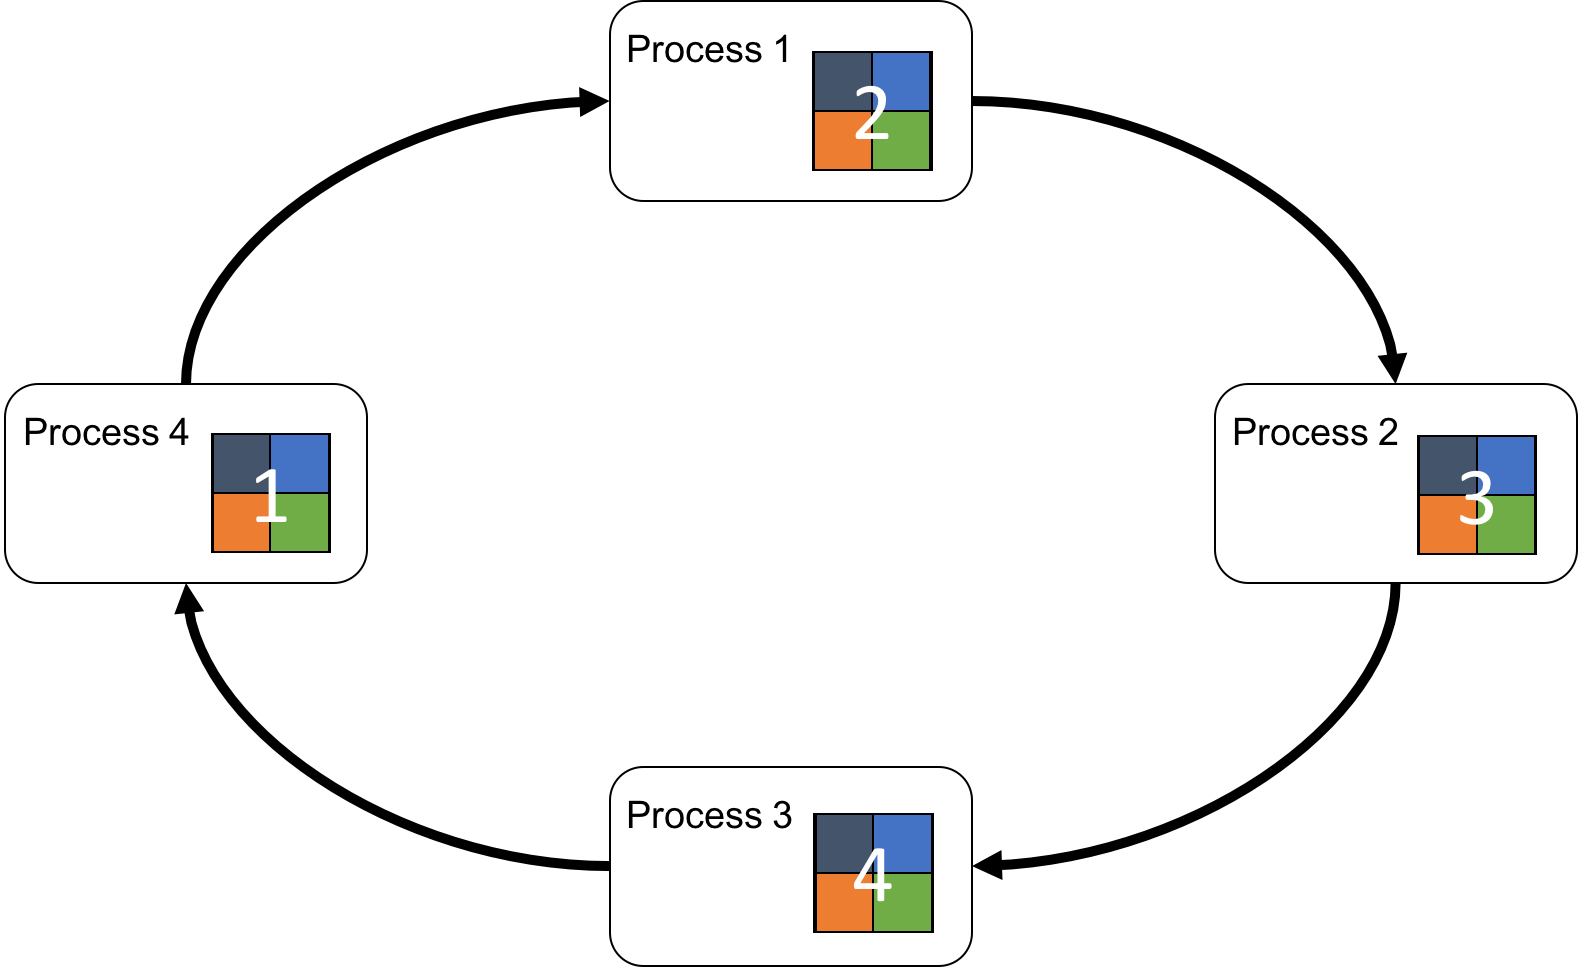
\includegraphics[width=0.48\textwidth]{imgs/nccl_topology_ring_tree_2.png}
        %\caption{Schema topologia ring/allreduce con peer-to-peer}
        \label{fig:ring-tree}
    \end{figure}
\end{frame}

\begin{frame}{Caratteristiche NCCL}{Prestazioni e Asincronicità}
    \begin{itemize}
        \item Comunicazioni asincrone: integrazione con CUDA stream.
        \item Overlapping tra computazione e comunicazione.
        \item Adattamento automatico all’hardware per ridurre latenza e aumentare il throughput.
        \item Ottimizzato per decine o centinaia di GPU.
    \end{itemize}
\end{frame}

\begin{frame}{Confronto con MPI}
    \begin{itemize}
        \item \textbf{Intra-nodo}: NCCL più performante grazie a NVLink e SHMEM.
        \item \textbf{Multi-nodo}: supporta RDMA via UCX/Infiniband.
        \item MPI è più flessibile (comunicazioni punto-a-punto), ma meno ottimizzato per GPU.
        \item NCCL ha un'API più semplice e orientata a CUDA.
    \end{itemize}
\end{frame}

\begin{frame}[fragile]{Esempio NCCL - AllReduce}
    \begin{itemize}
        \item Operazione di \texttt{all-reduce} tra più GPU:
    \end{itemize}

    \begin{lstlisting}[language=C++, basicstyle=\ttfamily\small, keywordstyle=\color{blue}]
        ncclAllReduce(sendbuff, recvbuff, count,
                    ncclFloat, ncclSum,
                    comm, stream);
    \end{lstlisting}

    \begin{itemize}
        \item Comunicazione asincrona rispetto all’host.
        \item \texttt{comm}: comunicatore NCCL. \texttt{stream}: CUDA stream associato.
    \end{itemize}
\end{frame}

\begin{frame}{Limiti e svantaggi}
    \begin{itemize}
        \item Overhead iniziale nella creazione dei comunicatori distribuiti.
        \item Flessibilità limitata: mancano comunicazioni punto-a-punto e topologie arbitrarie.
        \item Supportata solo su GPU NVIDIA e ambienti CUDA.
        \item Ottimale solo con reti ad alte prestazioni (NVLink, InfiniBand).
    \end{itemize}
\end{frame}

\begin{frame}{Applicazione a SUMMA con NCCL}
    \begin{itemize}
        \item NCCL può sostituire \texttt{MPI\_Bcast} per propagare pannelli $\mathbf{A}$ e $\mathbf{B}$.
        \item Due \texttt{ncclBroadcast} paralleli lungo righe e colonne della griglia.
        \item \texttt{ncclGroupStart/End} per gestire sincronizzazione e efficienza.
    \end{itemize}

    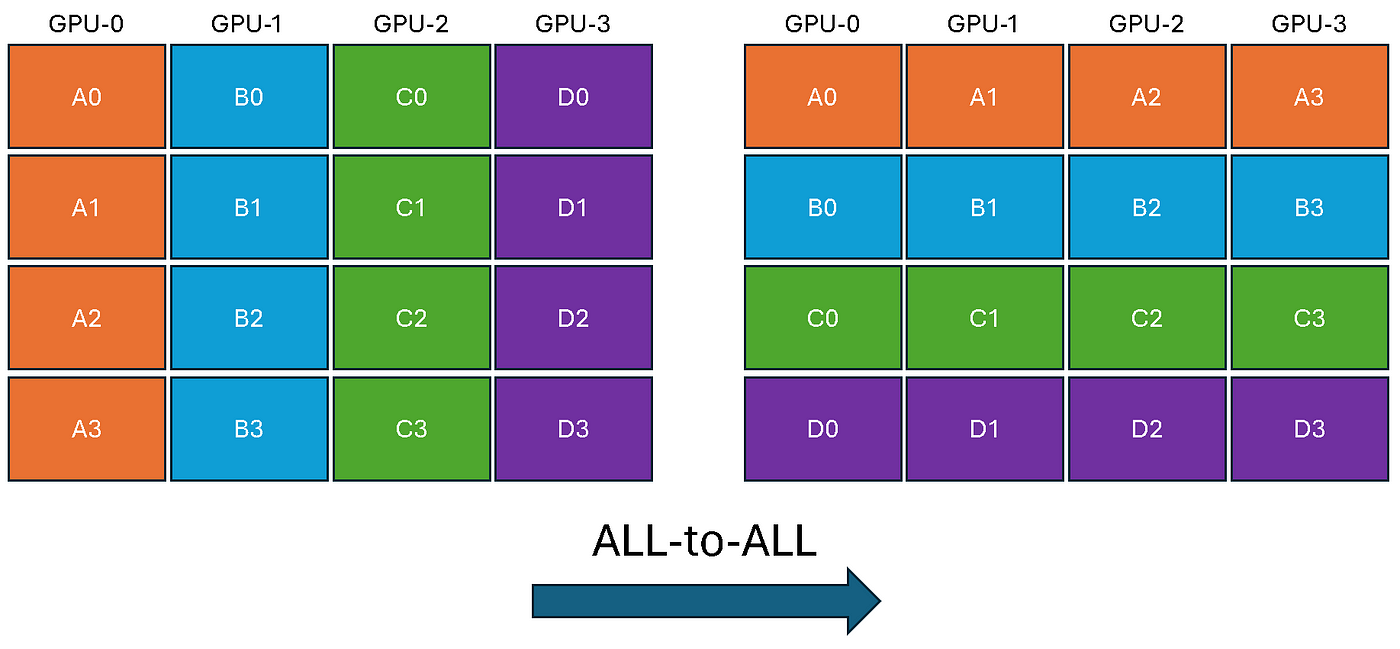
\includegraphics[width=0.6\textwidth]{imgs/summa_nccl.png}
    % TODO: Mostrare i due broadcast paralleli nella matrice
\end{frame}